\documentclass[tikz,border=5pt]{standalone}
\begin{document}
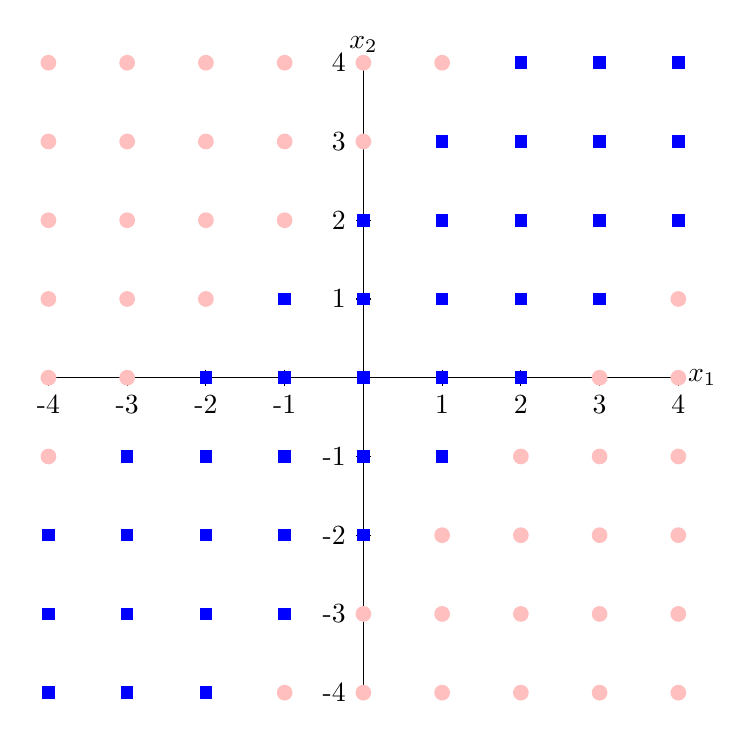
\begin{tikzpicture}[scale=1.0]

% Axes
\draw[->] (-4,0) -- (4,0) node[right] {$x_1$};
\draw[->] (0,-4) -- (0,4) node[above] {$x_2$};

% Axis ticks
\foreach \x in {-4,-3,-2,-1,1,2,3,4} {
  \draw (\x,0.1) -- (\x,-0.1) node[below] {\x};
}
\foreach \y in {-4,-3,-2,-1,1,2,3,4} {
  \draw (0.1,\y) -- (-0.1,\y) node[left] {\y};
}

% Grid of points
\foreach \x in {-4,-3,...,4} {
  \foreach \y in {-4,-3,...,4} {
    % Condition for class separation: between lines x2 = x1-2 and x2 = x1+2
    \pgfmathparse{(\y >= \x-2) && (\y <= \x+2)}
    \ifnum\pgfmathresult=1
      % inside margin band -> blue square
      \fill[blue] (\x-0.08,\y-0.08) rectangle (\x+0.08,\y+0.08);
    \else
      % outside band -> pink circle
      \fill[pink] (\x,\y) circle (0.1);
    \fi
  }
}

% Separating lines removed

\end{tikzpicture}
\end{document}